\documentclass[11pt,a4paper,vietnamese]{report}
\usepackage{babel}%sử dụng tiếng việt
\usepackage[margin=1in]{geometry}
\usepackage{amsfonts,amsmath,amssymb}%gói gõ công thức toán
\usepackage[none]{hyphenat}
\usepackage{fancyhdr}
\usepackage{graphicx}% thu vien anh
\usepackage{float}
\usepackage{subcaption}
\usepackage[nottoc,notlot,notlof]{tocbibind}
\usepackage{titlesec}
\usepackage{makeidx}

\pagestyle{fancy}
\fancyhead{}
\fancyfoot{}
\fancyhead[L]{\slshape\MakeUppercase{Floating point}}
\fancyhead[R]{\slshape{Van Duc NGUYEN}}
\fancyfoot[C]{\thepage}
%\renewcommand{\headrulewidth}{0pt}
\renewcommand{\footrulewidth}{0pt}

%\parindent 0ex
%\setlength{\parindent}{4ex}
%\setlength{\parskip}{1ex}
\renewcommand{\baselinestretch}{1.5}
\makeindex

\begin{document}
\begin{titlepage}
\begin{center}
\vspace*{1cm}
\Large\textbf{Floating point}\\
\large\textbf{Viettel IC Design}\\
\vfill
\line(1,0){400}\\[1mm]
\huge{\textbf{Floating point}}\\[3mm]
\Large{\textbf{-Floating point implement in FPGA-}}\\[1mm]
\line(1,0){400}\\
\vfill
By Van Duc NGUYEN\\
Candidate 20151050 \\
\today
\end{center}
\end{titlepage}
	
\tableofcontents
\listoffigures
\listoftables
\thispagestyle{empty}
\clearpage

\setcounter{page}{1}
\chapter{Introduction}
Ngày nay,trong các thế hệ chip xử lý việc tính toán hiệu năng cao là 1 yêu cầu cần thiết.Để thực hiện nhiệm vụ đó,rất nhiều hàm tính toán số học được thực hiện bên bộ xử lý của phần cứng nhanh hơn so với tính toán trên phần mềm trong cùng một nhiệm vụ.Những hoạt động chính của quá trình xử lý là tính toán các hàm số học,được ứng dụng rất rộng rãi trong tính toán khoa học,xủ lý ảnh và tín hiệu..Đăc biệt trong quá trình xử lý tín hiệu,các hàm tính toán cơ bản như cộng,nhân,chia được sử dụng rất rộng rãi trong nhiều ứng dụng.


Trong biểu diễn số học trong máy tính có 2 kiểu biểu diễn phổ biến,đó là kiểu fixed-point và kiểu floating-point.Với kiểu biểu diễn fixed-point(ví dụ:mã bù 2),hoàn toàn có thể biểu diễn các số nguyên dương và âm hoặc các số gần 0.Bằng cách cố định radix 2 hoặc radix cao hơn.Với kiểu định dạng này,có thể biểu diễn số với phần thập phân 1 cách dễ dàng.

Tuy nhiên,cách tiếp cận này có vài hạn chế.Không thể biểu diễn các số rất lớn hoặc các số rất nhỏ.Hơn nữa,phần thập phân của thương của 1 phép chia 2 số có thể bị mất mát.
Ví dụ với hệ thập phân,với số 976,000,000,000,000 có thể biểu diễn thành $9.76*10^{14}$,bằng cách biểu diễn như vậy,
có thể dễ dàng biểu diễn các giá trị rất lớn hoặc rất nhỏ trong các bộ nhớ có giói hạn trong các phần cứng.Việc sử dụng floating point giúp có thể tính toán trên dải rộng và độ chính xác cao.

Công việc trong báo cáo này bao gồm thiết kế và kiểm tra các phép toán số học cơ bản:cộng,nhân,chia,phép nghịch đảo và căn bậc 2 trên dấu phảy động.Cả đầu vào và đầu ra của các phép toán đều được thiết kế cho dấu phảy động với độ chính xác đơn theo tiêu chuẩn của IEEE 754/2008 cho dấu phảy động.
\chapter{Floating-point representation}

\section{Biểu diễn số floating-point}
Biểu thức biểu diễn dạng của số floating-point
\begin{center}
{$\pm{S}*B^{\pm{E}}$}\\
\end{center}
 1 số bất kỳ được biểu diễn dưới dạng cơ số B: nhị phân(hoặc thập phân) với 3 thành phần:
\begin{itemize}
\item Sign:phần dấu(cộng(+) hoặc trừ(-))
\item Significand S :phần định trị(còn có tên khác là mantissa hoặc fraction)
\item Exponent E : phần mũ.
\end{itemize}
\begin{center}
  \begin{figure}[htp]
  \begin{center}
  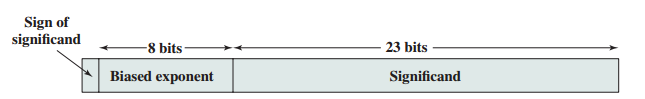
\includegraphics[scale=0.7]{image/fig1.png}
  \end{center}
  \caption{Định dạng của số 32-bit floating-point}
  \label{reffig1.png}
  \end{figure}
\end{center}
Trong công thức trên cơ số B được ẩn và không cần phải lưu trữ bởi vì nó dùng để biểu diễn cho toàn bộ số.Hình 2.1 biểu diễn định dạng của số 32-bit floating-point dạng cơ số 2,trong đó giá trị bit lớn nhất dùng để lưu trữ dấu của số cần biểu diễn(0= dương,1= âm).Giá trị phần mũ được lưu vào 8  bit tiếp theo,đây là kiểu biểu diễn BRN(biased representation number) với giá trị 1 giá trị cố định được gọi là bias,khi tính giá trị thật của số mũ cần biểu diễn ta lấy giá trị BRN trừ đi bias.Giá trị bias được tính theo công thức $(2^{k-1}-1)$,với k là số bit mà phần mũ biểu diễn dưới dạng binary(trong trường hợp này là 8 bit).Do đó dải sô mũ biểu diễn từ 0-255 tương ứng với dải biểu diễn của số mũ thật từ -127 đến +128.Phần bit còn lại(trong trường hợp này là 23 bit cuổi) là phần định trị(significand).
\subsection{Normalized,unnormalized and denormalized representation}
Số floating-point có nhiều cách biểu diễn khác nhau.ví dụ các giá trị dưới đây đều biểu diễn 1 số,nhưng số mũ và phần định trị khác nhau:
\begin{center}
$0.1101*2^6$\\
$1101*2^2$\\
$0.01101*2^7$\\
\end{center}
\subsubsection{Dạng chuẩn hóa(Normalized)}
Để đơn giản trong việc tính toán trên floating-point.Các số cần được chuẩn hóa về dạng:
\begin{center}
$\pm{1.mmm...m}*B^{\pm{E}}$\\
\end{center}
Với cơ số 2,biểu thức biểu diễn dạng chuẩn hóa là:
\begin{center}
$\pm{1.bbb...b}*2^{\pm{E}}$\\
\end{center}
Với b là số binary(0 hoặc 1).Bởi vì MSB(most significant bit) luôn là 1 nên không cần lưu trữ và được coi là bit ẩn(hidden bit).Vì vậy giá trị của phần định trị ở dạng chuẩn hóa nằm trong khoảng từ [1,2).\\
Hình 2.2 so sánh dải biểu diễn của kiểu fixed-point và floating point với cùng độ dài 32-bit.
\begin{center}
    \begin{figure}[htp]
    \begin{center}
     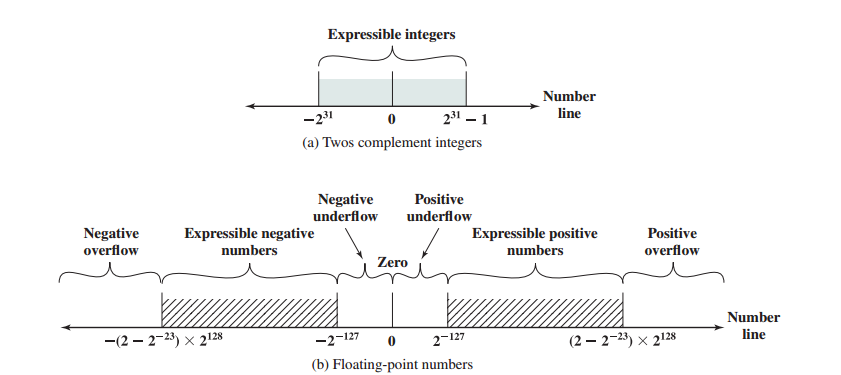
\includegraphics[scale=.5]{image/fig2.png}
    \end{center}
    \caption{Dải biểu diễn của fixed-point và floating trong định dạng 32-bit}
    \label{reffig2.png}
    \end{figure}
\end{center}
Với hình 2.2.a sử dụng kiểu biểu diễn mã bù 2(thuộc kiểu fixed-point),với dải biểu diễn từ $-2^{31}$ đến $2^{31}-1$ và tổng số biểu diễn được là $2^{23}$.Đối với số floating-point,dải biểu diễn được thể hiện trong hình 2.2.b:
\begin{itemize}
\item số âm nằm trong khoảng từ $-(2-2^{-23})*2^{128}$ đến $-2^{-127}$
\item số dương nằm trong khoảng từ $2^{-127}$đến $(2-2^{-23})*2^{128}$
\end{itemize}
Trong đó có 5 vùng không thuộc khoảng trên:
\begin{itemize}
\item các số âm nhỏ hơn $-(2-2^{-23})*2^{128}$ được gọi là negative overflow.
\item các số âm lớn hơn $-2^{-127}$ được gọi là negative underflow.
\item số 0
\item các số dương nhỏ hơn $2^{-127}$ được gọi là positive underflow.
\item các số dương lớn hơn $(2-2^{-23})*2^{128}$ được gọi là positive overflow.
\end{itemize}
Các số thuộc vùng negative underflow và positive underflow được gọi là unnormalized.

Giá trị \textbf{0} là giá trị đặc biệt mà kiểu biểu diễn sử dụng với phần định trị bằng 0 và phần mũ là giá trị nhỏ nhất của số mũ.
\subsubsection{Dạng chưa chuẩn hóa(Denormalized)}
Các số unnormalized được được chuẩn IEEE 754 quy định là số denormalized.Biểu thức của dạng biểu diễn denormalized:
\begin{center}
$\pm{0.mmm...m}*B^{E_{min}}$
\end{center}
Trong đó phần hidden bit chuyển từ \textbf{1.} sang \textbf{0.} .Và số mũ chỉ cho phép là số mũ nhỏ nhất.
\subsection{Biểu diễn phần định trị(Significand)}
Phần định trị là 1 số có dấu.Có 2 cách phổ biến để biểu diễn 1 số có dấu là sign-and-magnitude và 2's complement(mã bù 2).Hiện nay các biểu diễn sign-and-magnitude được dùng nhiều hơn vì nó biểu diễn số một cách tự nhiên và đơn giản khi thực hiện các hàm nhân,chia trên dấu phảy động.Với cơ số B=2,trong dạng chuẩn hóa bit lớn nhất của significand luôn là 1.Vì vậy nó không cần thiết được lưu trữ trong định dạng của kiểu biểu diễn.MSB của phần significand được gọi là \textbf{hidden bit}
\subsection{Biểu diễn phần mũ(Exponent)}
Phần mũ E là kiểu số nguyên có dấu,có thể biểu diễn bằng nhiều cách như sign-and-magnitude,
true-and-comlement,và biased.Cách biểu diễn biased được chọn bởi vì nó rất đơn giản khi so sánh 2 số floating-point và giá trị nhỏ nhất của số mũ là 0,vì vậy có thể biểu diễn giá trị 0 trong floating point.
Giá trị biểu diễn biased với bias là B,giá trị số mũ E được biểu diễn là số nguyên dương $E_R$:
\begin{center}
$E_R=E+B$
\end{center}
Giá trị nhỏ nhất của số mũ $E_R$=0,nên:
\begin{center}
$B=-E_{min}$
\end{center}
Dựa vào tính đối xứng của dải biểu diễn số mũ ta có:
\begin{center}
$-B\leq E\leq B$
\end{center}
Suy ra
\begin{center}
$0\leq E_R\leq 2B$
\end{center}
Với k là sô bit của kiểu biểu diễn binary của $E_R$:
\begin{center}
$2B\leq 2^k-1$
\end{center}
Cuối cùng ta được:
\begin{center}
$B\leq \frac{1}{2}(2^k-2)=2^{k-1}-1$
\end{center}
\subsection{Các giá trị đặc biệt}
Có một vài giá trị không biểu diễn được trong hệ thống floating-point nhưng nó rất cần thiết.Ví dụ như số vô cùng(infinity) hay NaN(Not a Number).Có nhiều phép toán mà khi thực hiện giá trị trả về không phải số ví dụ như phép căn bậc hai của một số âm,số vô cùng chia cho 0,hoặc kết quả ra là số vô cùng như phép chia cho 0...
\section{Các chế độ làm tròn và phân tích lỗi}
Có 4 chế độ làm tròn(Rounding) được IEEE quy định trong floating-point
\chapter{IEEE 754/2008 standard for binary floating-point}
Trong tiêu chuẩn IEEE 754/2008 có 2 tiêu chuẩn biểu diễn số floating-point dưới dạng cơ số 2 và cơ số 10.Trong báo cáo này đề cập tới việc biểu diễn số floating-point với cơ số 2.Tiêu chuẩn này được phát triển giúp cho sự chuyển đổi linh hoạt các chương trình từ một bộ xử lý này sang các bộ xử lý khác và được khuyên dùng trong pháp triển các chương trình tinh vi,định hướng số.
IEEE 754/2008 định ngĩa 3 kiểu định dạng floating-point khác nhau.
\begin{itemize}
\item Arithmetic format(Định dạng số học):Định dạng này có thể sử dụng để thể hiện biểu diễn dấu phảy động với các toán hạng hoặc kết quả sau khi thực hiện các hàm tính toán được mô tả trong tiêu chuẩn.
\item Basic format(Định dạng cơ bản):Định dạng này bao gồm 5 kiểu kiểu diễn dấu phảy động( 3 kiểu nhị phân và 2 kiểu cho thập phân).Và được mã hóa theo tiêu chuẩn ,được sử dụng cho tính toán số học.
\item Interchange format(Định dạng trao đổi):Mã hóa nhị phân có độ dài cố định,đầy đủ cho phép trao đổi dữ liệu giữa các nền tảng khác nhau và có thể được sử dụng để lưu trữ.
\end{itemize}
\section{Tiêu chuẩn IEEE 754/2008 cho floating-point binary.}
Có 3 định dạng cơ bản của dấu phảy động nhị phân với chiều dài bit là 32,64 và 128 bit,tương ứng với độ rộng của số bit lần lượt là 8 bit,11 bit và 15 bit.(2 định dạng cơ bản còn lại cho dấu phảy động thập phân với độ dài bit là 64 và 128 bit).Tất cả các định dạng cơ bản cũng đồng thời là định dạng số học(được sử dụng cho tính toán số học) và định dạng trao đổi.
Ngoài ra còn có vài định dạng cho ứng dụng chuyên biệt như định dạng 16 bit nhi phân khi tính toán không yêu cầu độ chính xác cao.Hoặc định dạng với độ chính xác mở rộng dành cho ứng dụng yêu cầu độ chính xác cao.
\begin{center}
    \begin{figure}[htp]
    \begin{center}
     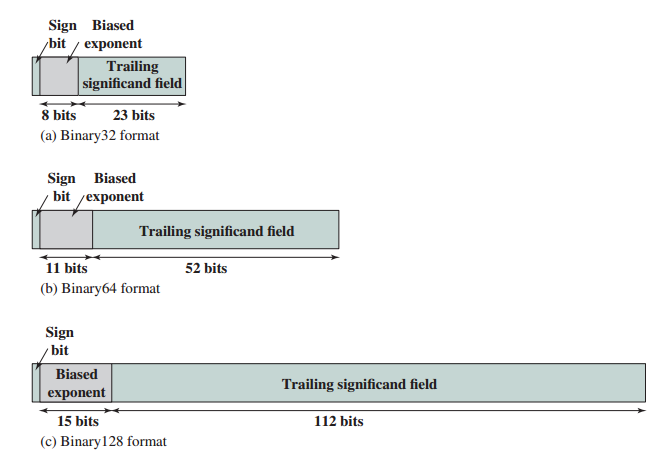
\includegraphics[scale=.7]{image/fig3}
    \end{center}
    \caption{Định dạng IEEE 754}
    \label{reffig3}
    \end{figure}
\end{center}
Hình 3.1 thể hiện định dạng IEEE 754 cho độ dài bit lần lượt là 16 bit(single precision),32bit(double precision),128 bit.
\begin{center}
    \begin{figure}[htp]
    \begin{center}
     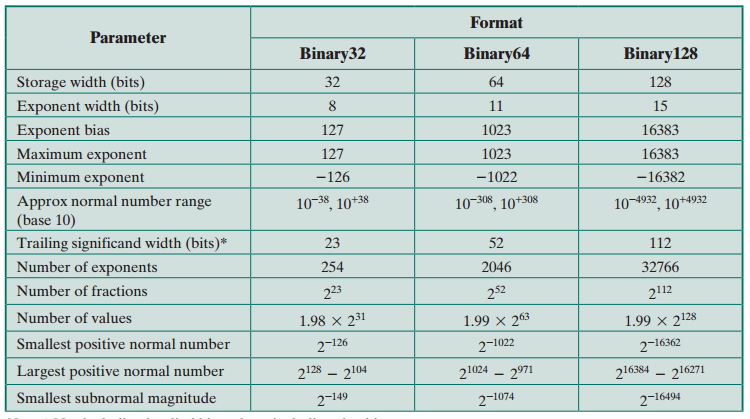
\includegraphics[scale=.7]{image/fig4}
    \end{center}
    \caption{Thông số của định dạng IEEE 754}
    \label{reffig4}
    \end{figure}
\end{center}
Hình 3.2 thể hiện mối quan hệ giữa cách kiểu định dạng với độ dài bit khác nhau.\\
Không phải tất cả các mẫu bit trong định dạng của IEEE 754 đều được giải thích theo cách thông thường,thay vào đó có một vài mẫu bit được sử dụng để biểu diễn giá trị đặc biệt.
\begin{center}
    \begin{figure}[htp]
    \begin{center}
     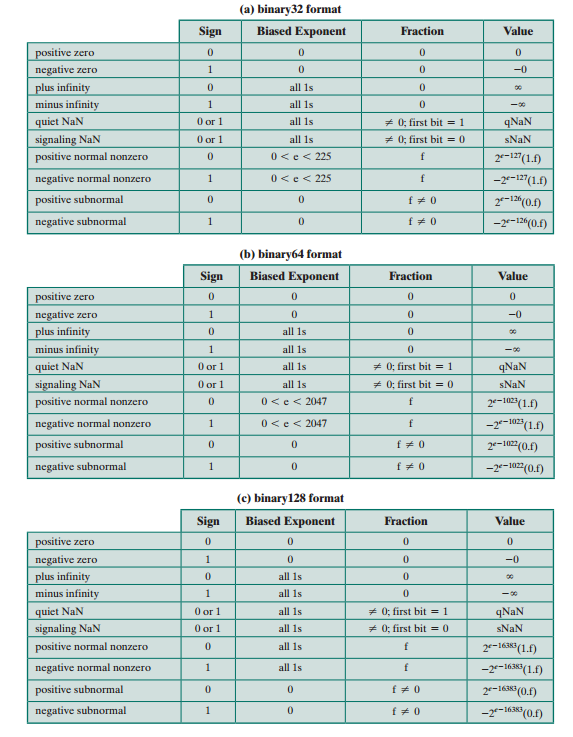
\includegraphics[scale=.8]{image/fig5}
    \end{center}
    \caption{Các trường hợp biểu diễn trong IEEE 754 floating-point}
    \label{reffig5}
    \end{figure}
\end{center}
Hình 3.3 thể hiện sự phân chia thành các lớp mà số floating-point biểu diễn:
\begin{itemize}
\item Để biểu diễn số chuẩn hóa(normailzied),giá trị của số mũ E trong dải (0,255)đối với định dạng 32-bit,đối với 64-bit là từ $\left(0,2047\right)$và nằm trong dải(0,16383) đối với định dạng 64-bit.Giá trị thực của số mũ đã được hiệu chỉnh lệch đi một lượng bias,ví dụ dải thực của số mũ trong định dạng 32-bit là $\left[-126,127\right]$.Đồng thời khi ở dạng normalized yêu cầu bit \textbf{1} ở bên trái binary point(\textbf{1.}).Bit này được ẩn và là bit MSB(most significand bit) đối với phần định trị(mantissa hay fraction).
\item Để biểu diễn số \textbf{0},phần mũ E=0 và phần định trị F=0,dấu $\pm0$ được quyết định bởi bit dấu(sign bit).
\item Để biểu diễn số $\infty$ thì tất cả bit của phần mũ E đều bằng 1(Max E) và phần định trị(fraction)F=0.Dấu $\pm\infty$ phụ thuộc vào bit dấu S.
\item Để biểu diễn số chưa được chuẩn hóa(denormalized) thì phần mũ E=0 và phần định trị F $\neq0$.Trong trường hợp này số mũ thực mà số floating-point biểu diễn là -126(đối với 32-bit) và -1022(đối với 64-bit).Dấu của số phụ thuộc vào bit dấu S.
\item Đối với giá trị NaN(Not a Number),tất cả các bit của phần mũ E đều bằng 1(Max E) và phần định trị F$\neq0$.
\end{itemize}
\section{Các chế độ làm tròn trong tiêu chuẩn IEEE 754/2008 cho floating-point bianry}
Khi thực hiện các phép toán số học,kết quả số có thể được lưu trữ,bị dịch đi..Khi đưa về định dạng của số floating-point có thể bị cắt bỏ hoặc làm tròn tới giá trị chính xác gần nhất.Tiêu chuẩn của IEEE đưa ra 4 chế độ làm tròn:
\begin{itemize}
\item Round to nearnest:làm tròn về số gần nhất.
\item Round toward $+\infty$:làm tròn lên(tiến tới dương vô cùng).
\item Round toward  $-\infty$:làm tròn xuống(tiến tới âm vô cùng).
\item Round toward 0:làm tròn về gần 0.
\end{itemize}
Trong đó,chế độ làm tròn mặc địch được quy định là Round to nearnest.Kết quả sau khi được chuẩn hóa(normalized) có dạng $\textbf{1.}f_1f_2...f_l\textbf{RS}$
\begin{itemize}
\item $f_l$:(last fraction bit)là bit cuối cùng của phần định trị theo định dạng(bit thứ 23 đối với định dạng floating-point 32-bit).
\item R:(round bit)là bit đầu tiên sau bit $f_l$.
\item S:(sticky bit)xuất hiện sau round bit(được tính bằng phép OR các bit còn lại).
\end{itemize}
4 trường hợp của \textbf{RS}:
\begin{enumerate}
\item \textbf{RS}=00:Kết quả đã chính xác,không cần làm tròn.
\item \textbf{RS}=01:làm tròn kết quả xuống bằng cách cắt bỏ phần RS.
\item \textbf{RS}=11:làm tròn kết quả lên bằng cách cộng thêm 1 vào $f_l$.
\item \textbf{RS}=10:tăng hoặc giảm phụ thuộc vào $f_l$
\begin{itemize}
\item $f_l$=0:làm tròn kết quả xuống bằng cách cắt bỏ phần RS.
\item $f_l$=1:làm tròn kết quả lên bằng cách cộng thêm 1 vào $f_l$.
\end{itemize}
\end{enumerate}
\chapter{Floating-point arithmetic}
\section{Addition and Subtraction}
Phép cộng và phép trừ trong floating-point có chunng cách thực hiện(khi thực hiện phép trừ chỉ cần đảo dấu của 1 toán hạng và sử dụng phép cộng).
Với đầu vào là 2 số floating-point X($S_X,E_X,F_X$)và Y($S_Y,E_Y,F_Y$).Kết quả sau khi thực hiện phép toán X+Y là Z($S_Z,E_Z,F_Z$).\\
Các bước thực hiện phép toán cộng/trừ dấu phảy động:
\begin{enumerate}
\item Tách đầu vào thành 3 phần:phần dấu(sign),phần mũ(expoent) và phần định trị(mantissa).Kiểm tra đầu vào xem có thuộc các trường hợp đặc biệt như là số vô cùng,là số 0 hoặc số không hợp lệ theo chuẩn biểu diễn IEEE 754.Thêm bit ẩn vào phần định trị.
\item So sánh sô mũ của 2 số đầu vào:số nhỏ hơn sẽ bị dịch phải phần định trị để 2 số có cùng số mũ.Số bit dịch của phần định trị phụ thuộc vào sự sai khác giữa 2 số mũ.Sau đó cộng hoặc trừ phần định trị mới với mantissa của số lớn hơn.
\item Thực hiện phép dịch trái phần mantissa cho tới khi bit MSB bằng 1.Với mỗi lần dịch,giảm giá trị phần mũ đi 1.Làm tròn phần định trị nếu cần thiết.Cuối cùng đóng gói phần dấu,phần mũ và phần định trị theo định dạng và đưa ra kết quả
\end{enumerate}
Mã giả(pescode) của phép toán cộng 2 số floating-point.\\
bảng thể hiện giá trị phần dấu,mũ và mantissa của đầu ra theo đầu vào.\\
Sơ đồ khối thuật toán cộng 2 số dấu phảy động.
\section{Multiplication and Divison}

\section{Reciprocal and Square Root}

\chapter{Implement in FPGA}
\section{Addition and Subtraction}
\section{Multiplication and Division}
\section{Reciprocal and Square Root}
\chapter{Evaluation}

\chapter{Conclussion and Related-work}
This is end of document

\cite{name1}\\

\pagebreak
\begin{thebibliography}{}
\bibitem{name1}
Duc Nguyen,"sach cua toi",\textit{bai bao} Sun,25,May,2019.
\bibitem{name2}
Authors
\textit{"title of article"}
Title of Journal
Date,Month,Year
page
Medium of publish
\end{thebibliography}
\end{document}